\chapter{Architectural Design}
This section aims to present and analyze the architecture of the S2B in a top-down manner. 
We discuss about the architectural design choices and the reasons behind them. 

\section{Overview: High-level components and their interactions}
The figure shown below represents a high-level description of the components which make up the system.
\begin{figure}[H]
    \centering
    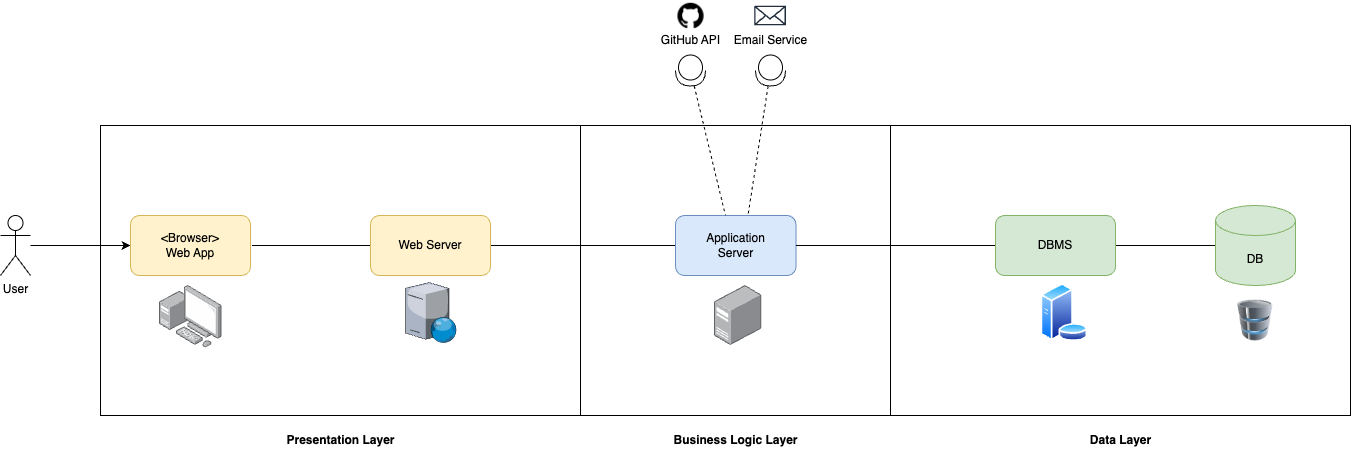
\includegraphics[width=\textwidth]{images/component_view/high_level.png}
    \caption{Overview CKB architecture}
    \label{fig:CKB Architecture}
\end{figure}
A web interface will be used to access the platform. 
The overall architecture of the system is based on a three-tier architecture, 
with the application servers interacting with a database management system and
using APIs to retrieve and store data. \\
The three logical layers correspond to three different physical layers and each layer can communicate only with the adjacent ones.
The interactions between clients and server are stateless according to the REST architectural style. \\
The web server is responsible for the communication with the clients and for the management of the requests. \\
The application server holds the business logic of the application and it can communicate with the database server to retrieve and store data, also with the GitHub platform and the Email Service. 

\section{Component view}

\subsection{High level view}
\begin{figure}[H]
    \centering
    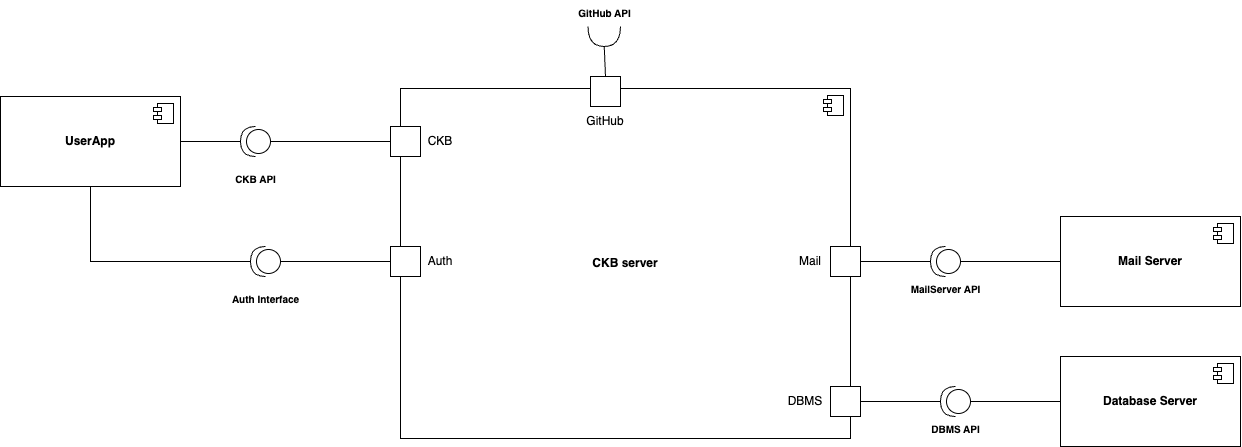
\includegraphics[width=\textwidth]{images/component_view/Component_view.png}
    \caption{High level component view}
\end{figure}
The figure above shows the system components and interfaces at a high level.
\begin{itemize}
    \item \textbf{CKBServer: } it represents the core of the CKB system and it contains all the business logic.
    \item \textbf{UserApp: } it represents the web application used by the users to access the CKB platform. Users register and log into the system through the 
    \textbf{AuthInterface} and access the functionalities offered by the system through the \textbf{CKB API}.
    \item \textbf{DatabaseServer: } it represents the DBMS used to store the data of the system. The system can access the data through the \textbf{DBMS API}.
    \item \textbf{MailServer: } it represents the mail server used to send notifications to the users. The system can access the mail server through the \textbf{MailServer API}.
\end{itemize}

\subsection{CKB Server detailed view}
\begin{figure}[H]
    \centering
    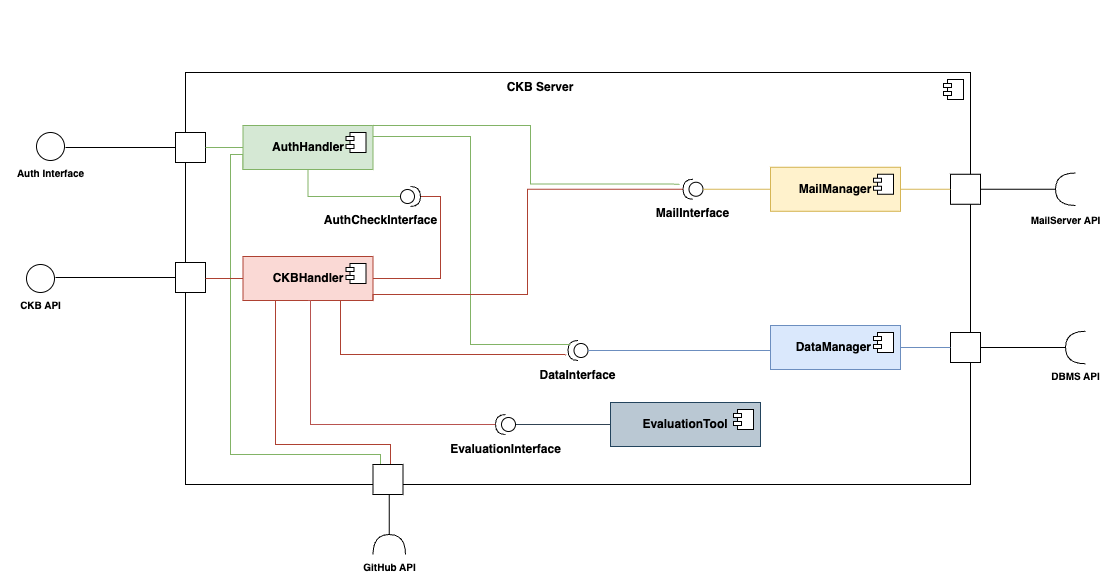
\includegraphics[width=\textwidth]{images/component_view/CKB_component.png}
    \caption{CKB server component view}
\end{figure}
The figure above shows the internal components of the CKB server.
\begin{itemize}
    \item \textbf{AuthHandler: } it handles the login and registration of the users. It offers the \textbf{AuthCheckInterface} to allow other components to check 
    if a user is authorized. It communicates with the \textbf{MailInterface} to manage confirmation emails and with the \textbf{DataInterface} to check the credentials
    correctness.
    \item \textbf{CKBHandler: } it handles all the functionalities offered by the system. It communicates with the \textbf{DataInterface} to retrieve and store data, with 
    the \textbf{AuthCheckInterface} to check if a user is authorized to perform a certain operation, with the \textbf{MailInterface} to send notifications to the users, and with
    the \textbf{EvaluationInterface} to perform the evaluation of the students' projects.
    It also communicates with the \textbf{GitHubInterface} to retrieve data (nickname and pushed code) from the GitHub platform.
    \item \textbf{MailManager: } it handles the access to the mail server, it provides the \textbf{MailInterface} that allows components to send emails.
    \item \textbf{DataManager: } it handles the access to the persistent data saved on the DB, almost every component communicates with it through the \textbf{DataInterface}.
    \item \textbf{EvaluationTool: } it handles the evaluation of the students' code based on the battle rules. It retrieves this information from the \textbf{CKBHandler}.
\end{itemize}


\subsection{Auth component view}
\begin{figure}[H]
    \centering
    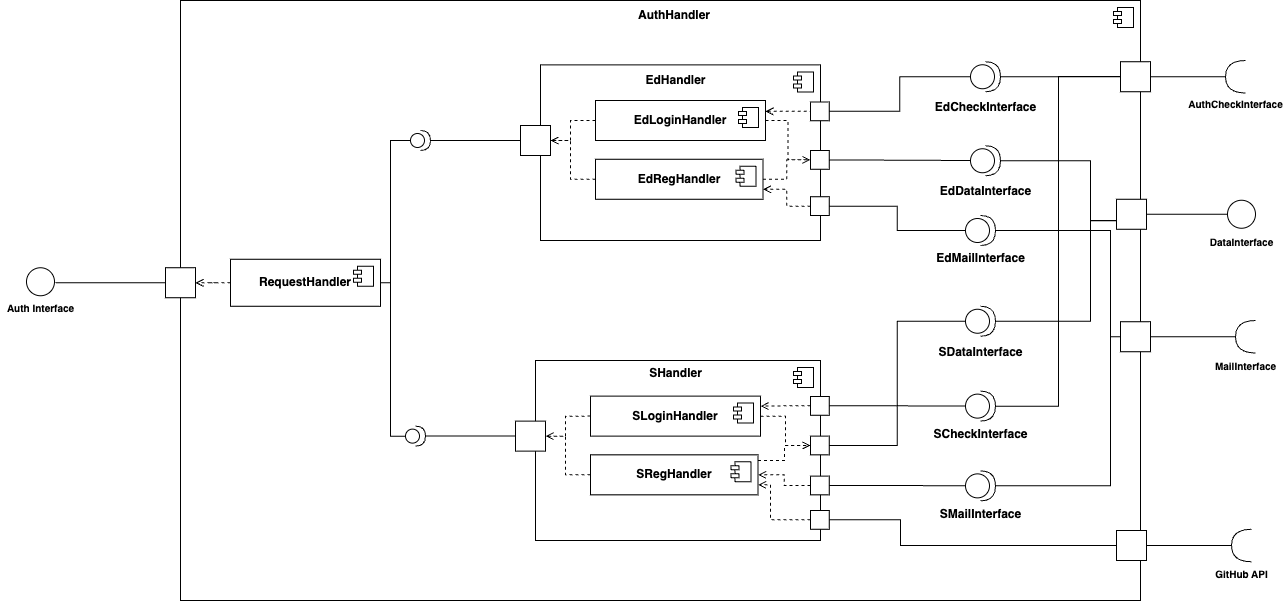
\includegraphics[width=\textwidth]{images/component_view/Auth.png}
    \caption{Auth component view}
\end{figure}
The figure above shows the internal components of the AuthHandler.
\begin{itemize}
    \item \textbf{RequestHandler: } it handles the requests acting as a router dispatching requests to the right handler.
    \item \textbf{EdHandler: } it is composed of the \textbf{EdLoginHandler} and the \textbf{EdRegHandler}. The former handles the login of educators, 
    the latter handles their registration.
    \item \textbf{SHandler: } it is composed of the \textbf{SLoginHandler} and the \textbf{SRegHandler}. The former handles the login of students,
    the latter handles their registration.
\end{itemize}
LoginHandlers communicate with the \textbf{AuthCheckInterface} to check the authorization of a user.\\
RegistrationHandlers communicate with the \textbf{MailInterface} to send confirmation emails and with the \textbf{DataInterface} to store the data of the new user.\\
SRegistrationHandler also communicate with \textbf{GitHubAPI} to link the CKB account with the GitHub one.

\subsection{CKB component view}
\begin{figure}[H]
    \centering
    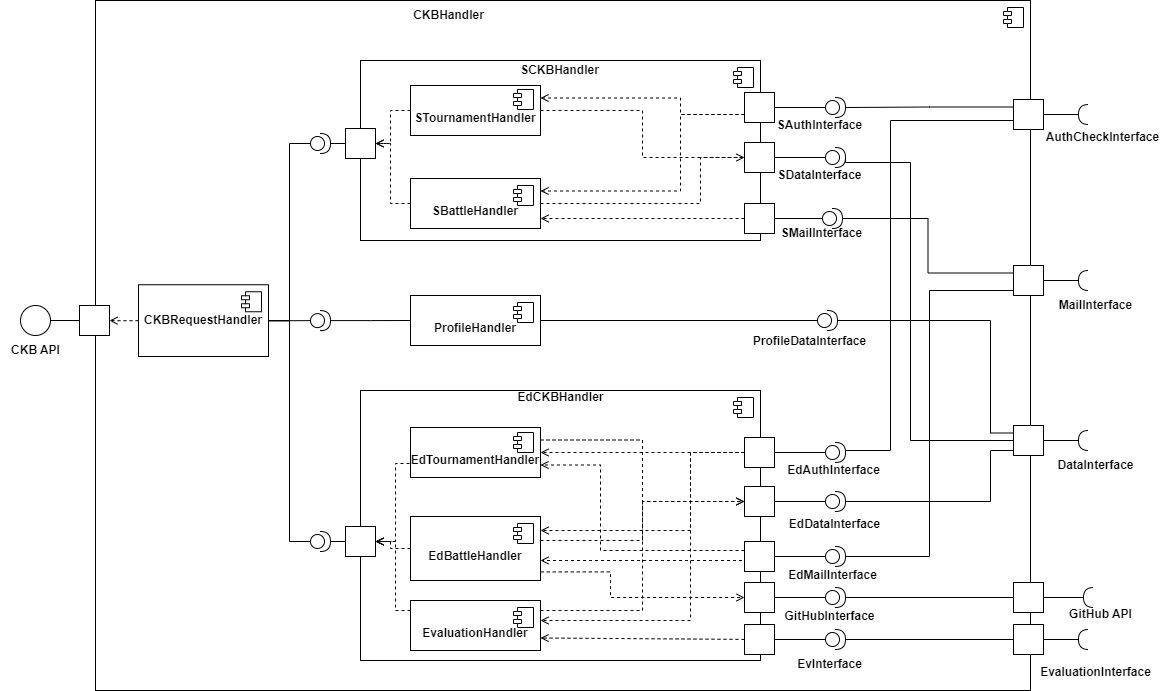
\includegraphics[width=\textwidth]{images/component_view/ckb_handler.png}
    \caption{CKB component view}
\end{figure}
The figure above shows the internal components of the CKBHandler.
\begin{itemize}
    \item \textbf{CKBRequestHandler: } it handles the requests acting as a router dispatching requests to the right handler.
    \item \textbf{EdCKBHandler: } it is composed of the \textbf{EdTournamentHandler}, the \textbf{EdBattleHandler} and the \textbf{EvaluationHandler}.
    EdTournamentHandler is responsible for the creation and the conclusion of tournaments, EdBattleHandler is responsible for the creation of battles, and 
    EvaluationHandler is responsible for the evaluation of the students' code.
    \item \textbf{SCKBHandler: } it is composed of the \textbf{STournamentHandler} and the \textbf{SBattleHandler}. STournamentHandler is responsible for the 
    visualization and the subscription to tournaments, SBattleHandler is responsible for the subscription to battles.
    \item \textbf{ProfileHandler: } it is responsible for the visualization of the profile of a student. 
\end{itemize}
All components communicate with the \textbf{AuthCheckInterface} to check the authorization of a user to perform the requested operation.\\
TournamentHandlers and BattleHandlers communicate with the \textbf{DataInterface} to retrieve and store data and with the \textbf{MailInterface} to send notifications to the users.\\
EdBattleHandler also communicates with the \textbf{GitHubAPI} to retrieve the students' pushed code.\\
EvaluationHandler communicates with the \textbf{EvaluationInterface} to evaluate the students' code and with the \textbf{DataInterface} to store the results of the evaluation.\\
ProfileHandler communicates with the \textbf{DataInterface} to retrieve the data of the searched student.


\section{Deployment view}
The figure below shows the architecture of the system. All the users access to the WebApp through the browser, which communicates with
the Web Server. Both Web Server and Application Server are hosted on a Cloud Provider. This choice offers many
advantages, such as:

\begin{itemize}
    \item  \textbf{Scalability and flexibility: }the ability of adding and removing resources efficiently through 
    the use of load balancing services which allow the application server to manage traffic and workload. 
    \item   \textbf{Security: }the ability to protect the application server using firewall and DMZ, against cyber attacks and possible threats.
    \item   \textbf{Cost efficiency:} the ability to pay only for the resources used which can help to lower the overall cost. 
\end{itemize}

\begin{figure}[H]
    \centering
    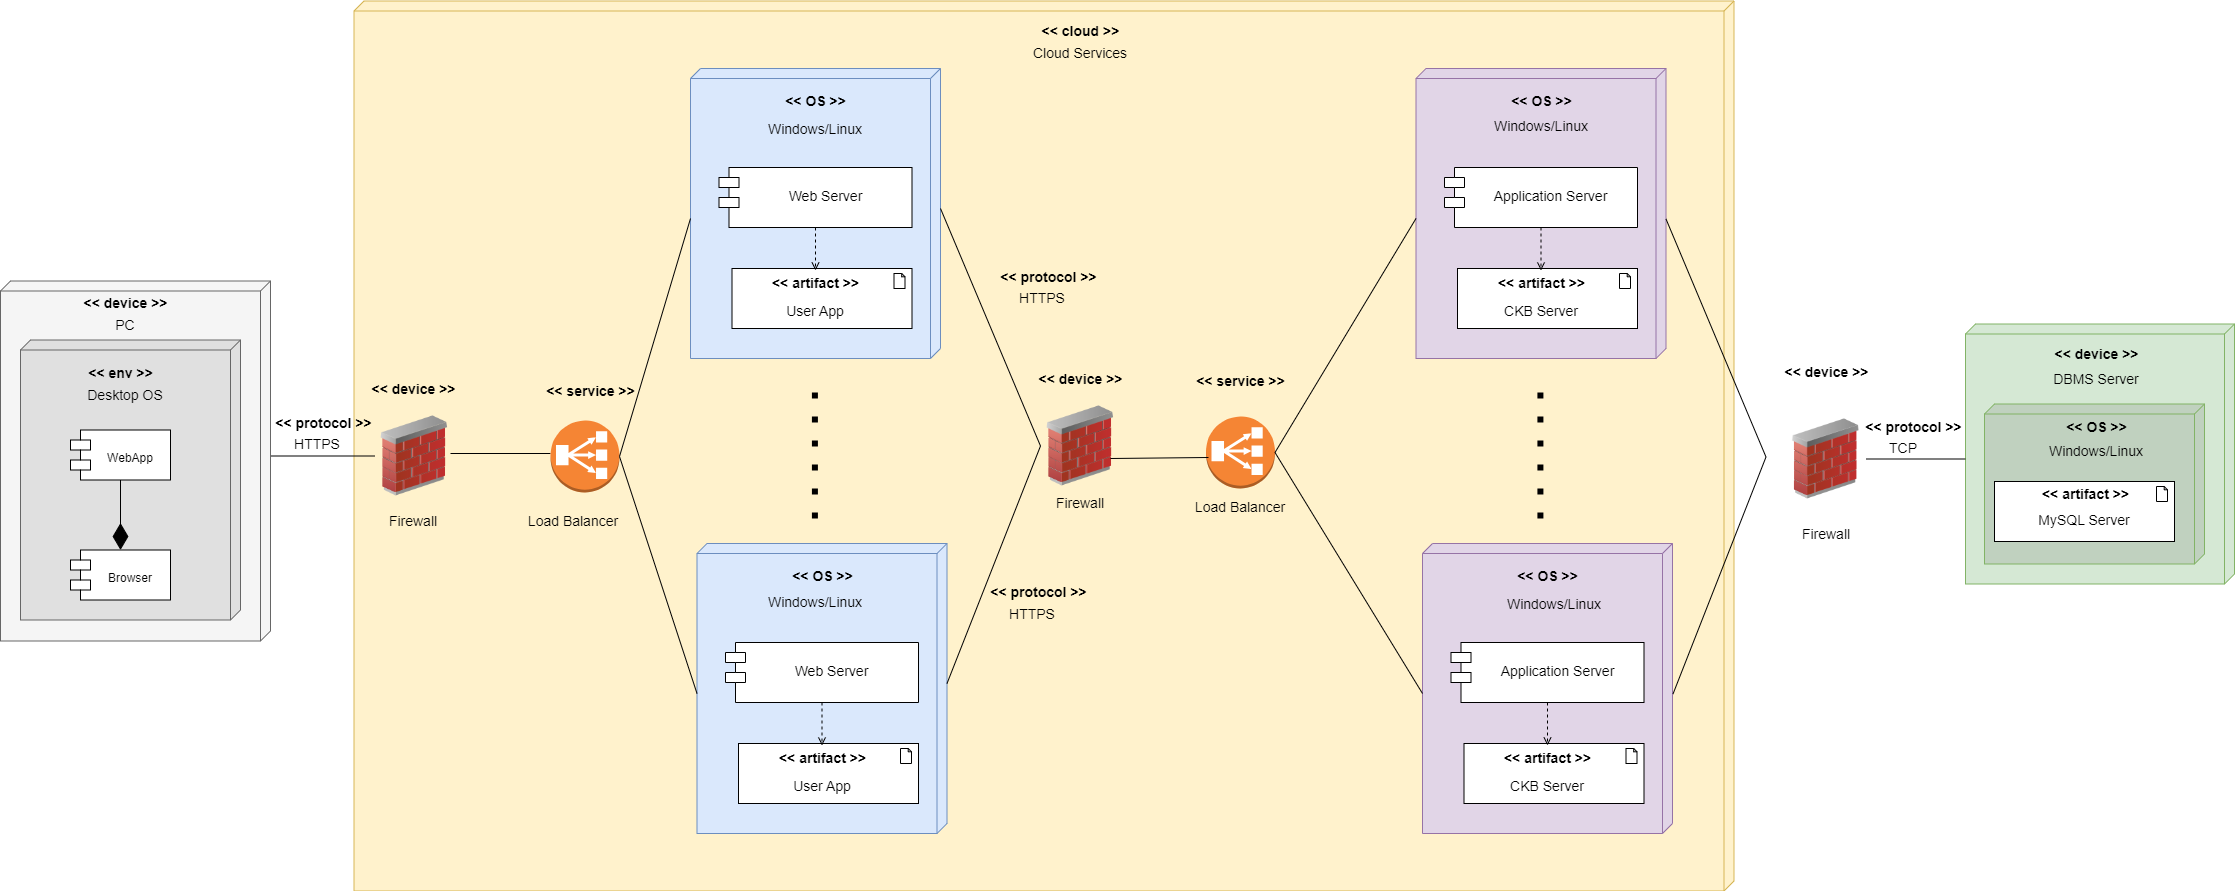
\includegraphics[width=1\textwidth]{images/Deployment_diagram.png}
    \caption{Deployment diagram}
\end{figure}

The deployment diagram offers a more detailed view over the hardware and software components of the system. 
\begin{itemize}
    \item  \textbf{PC: }any device having a browser capable of running the JavaScript code.
    \item   the Cloud Services will host all the business and data logic for the system. It is characterized by 
    \begin{itemize}
        \item  \textbf{Firewall:} device used to protect and filter incoming connections to the logic and data layers of the system. It protects the system from unauthorized access and malicious attacks.
        \item  \textbf{Load Balancer:} service used to distribute the workload across multiple servers. It helps to improve the performance and reliability of the system. It also helps to ensure that application can handle a large volume of requests, without any downtime.
        \item  \textbf{Multiple copies of Web Server and Application Server:} they are used to ensure that the system is always available. The different instances can be created and destroyed dynamically, based on the workload. It also helps to achieve fault tolerance by allowing traffic to be redirect to a different instance, if one instance becomes unavailable.
    \end{itemize}
    \item   \textbf{Database:} used to store all the data of the system. It uses MySQL as DBMS to retrieve and store data.
    \item   \textbf{Mail Provider: } used to send notifications to the users. It uses Gmail as mail provider.
\end{itemize}

\section{Runtime view}
\subsection{Registration Student}
The figure below shows the sequence diagram of the registration of a student. The student fills the form with their email and password and submits it. 
The database checks if the email is already used, if not the system sends a confirmation email to the student to complete the registration. 
The student inserts their personal information (name, surname, date of birth) and also their GitHub nickname. 
The system checks if the GitHub nickname is valid, if so the system saves the student's credentials and the registration is completed.\\

\begin{figure}[H]
    \centering
    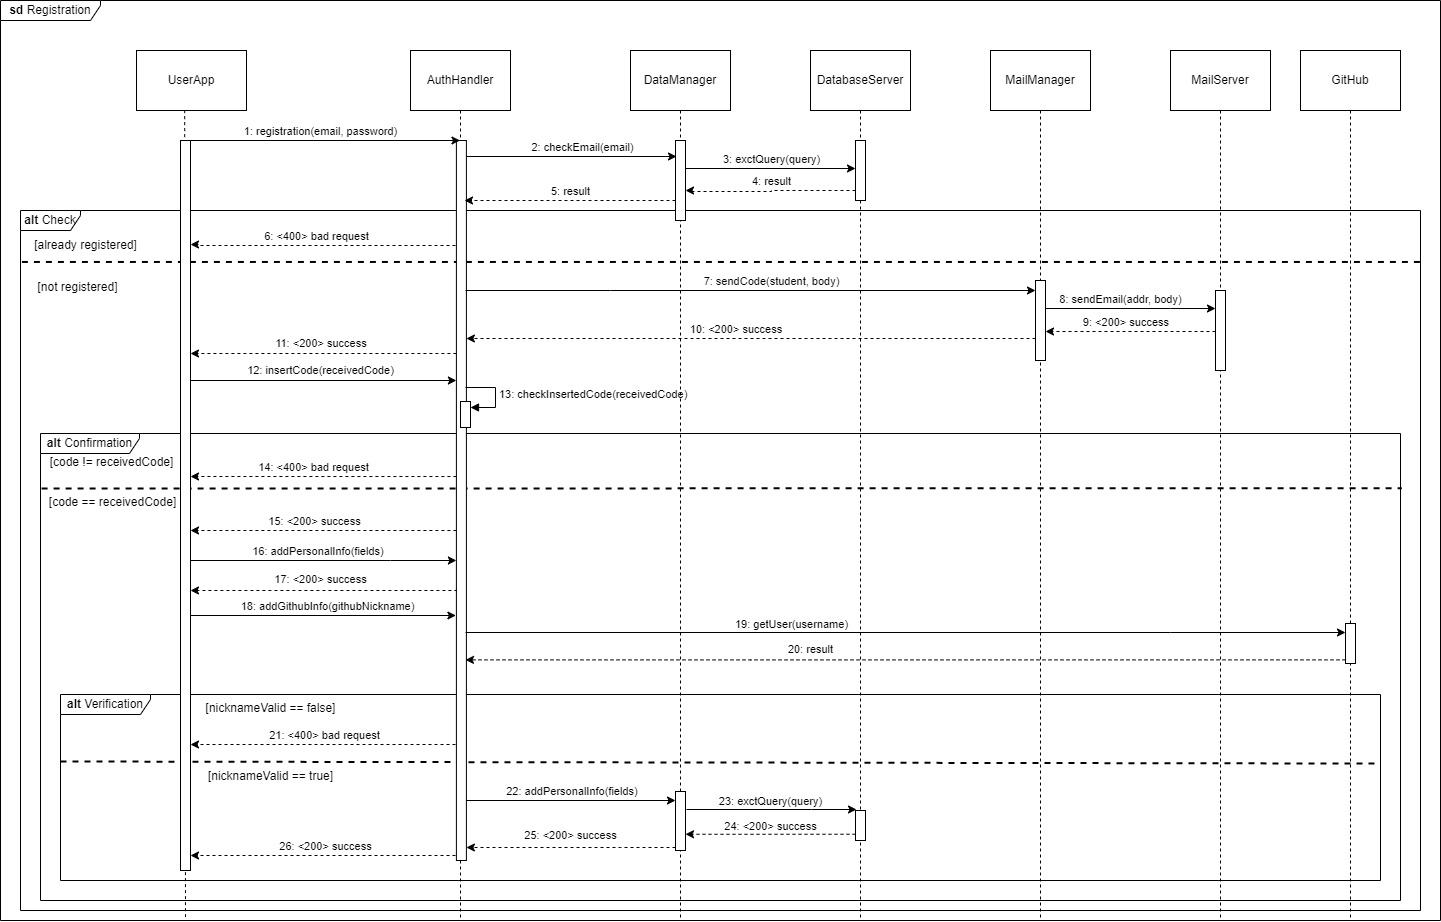
\includegraphics[width=1\textwidth]{images/seq_diagrams/RegistrationStd_DD.png}
    \caption{Registration Student}
\end{figure}
\clearpage

\subsection{Registration Educator}
The figure below shows the sequence diagram of the registration of an educator. The educator fills the form with their email and password and submits it. 
The database checks if the email is already used, if not the system sends a confirmation email to the educator to complete the registration. 
The educator inserts their personal information (name, surname, date of birth) and the system saves the educator's credentials and the registration is completed.\\
\begin{figure}[H]
    \centering
    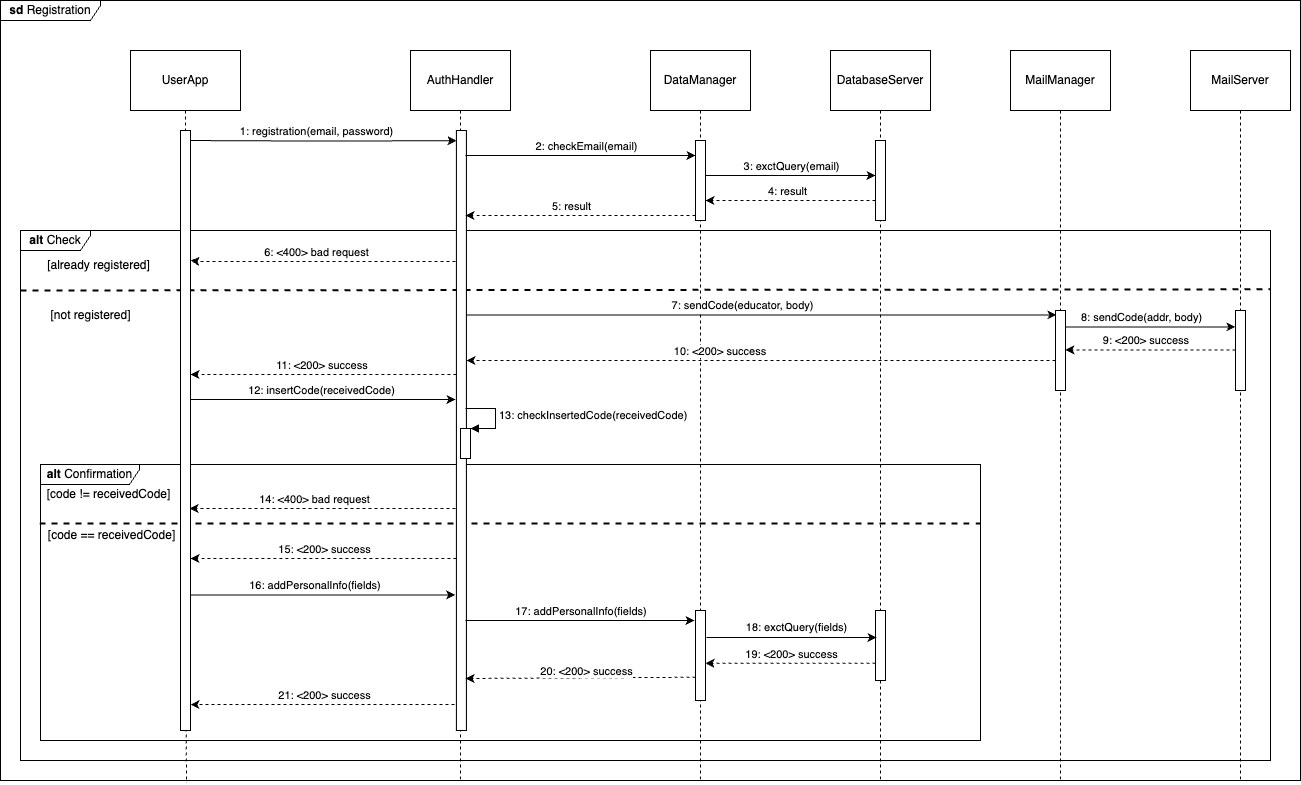
\includegraphics[width=1\textwidth]{images/seq_diagrams/RegistrationEd_DD.png}
    \caption{Registration Educator}
\end{figure}
\clearpage

\subsection{Login}
The figure below shows the sequence diagram of the user login. The user fills the form with their email and password and submits it. 
The system checks if the credentials are stored and valid, if so the user is logged in, otherwise the system shows an error message.\\
\begin{figure}[H]
    \centering
    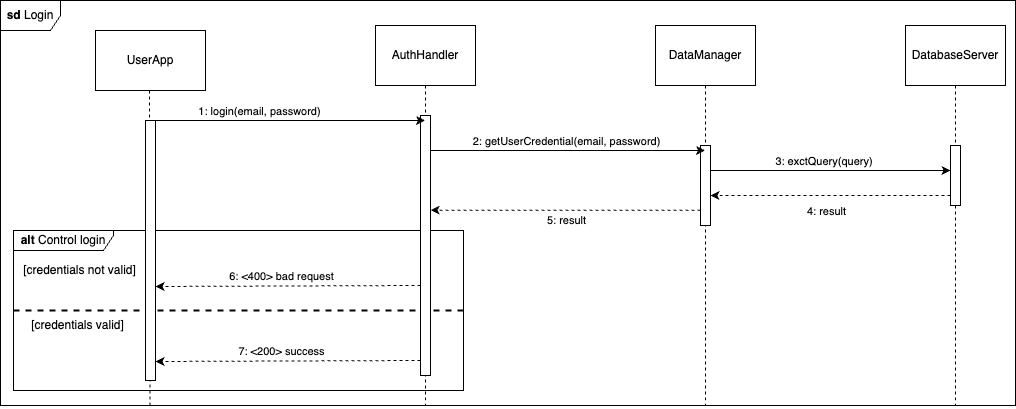
\includegraphics[width=1\textwidth]{images/seq_diagrams/Login_DD.png}
    \caption{Login}
\end{figure}
\clearpage

\subsection{Creation of the tournament}
The figure below shows the sequence diagram of the creation of a tournament. The educator fills the form
 with the tournament details and submits it. The system checks if the data is valid, and if the badge option is set to true, the system creates the badge.
 After that the system sends an email to all the invited colleagues and to all the students subscribed to the CKB platform. 
 The tournament is created and the educator is redirected to the tournament page.\\

 \begin{figure}[H]
    \centering
    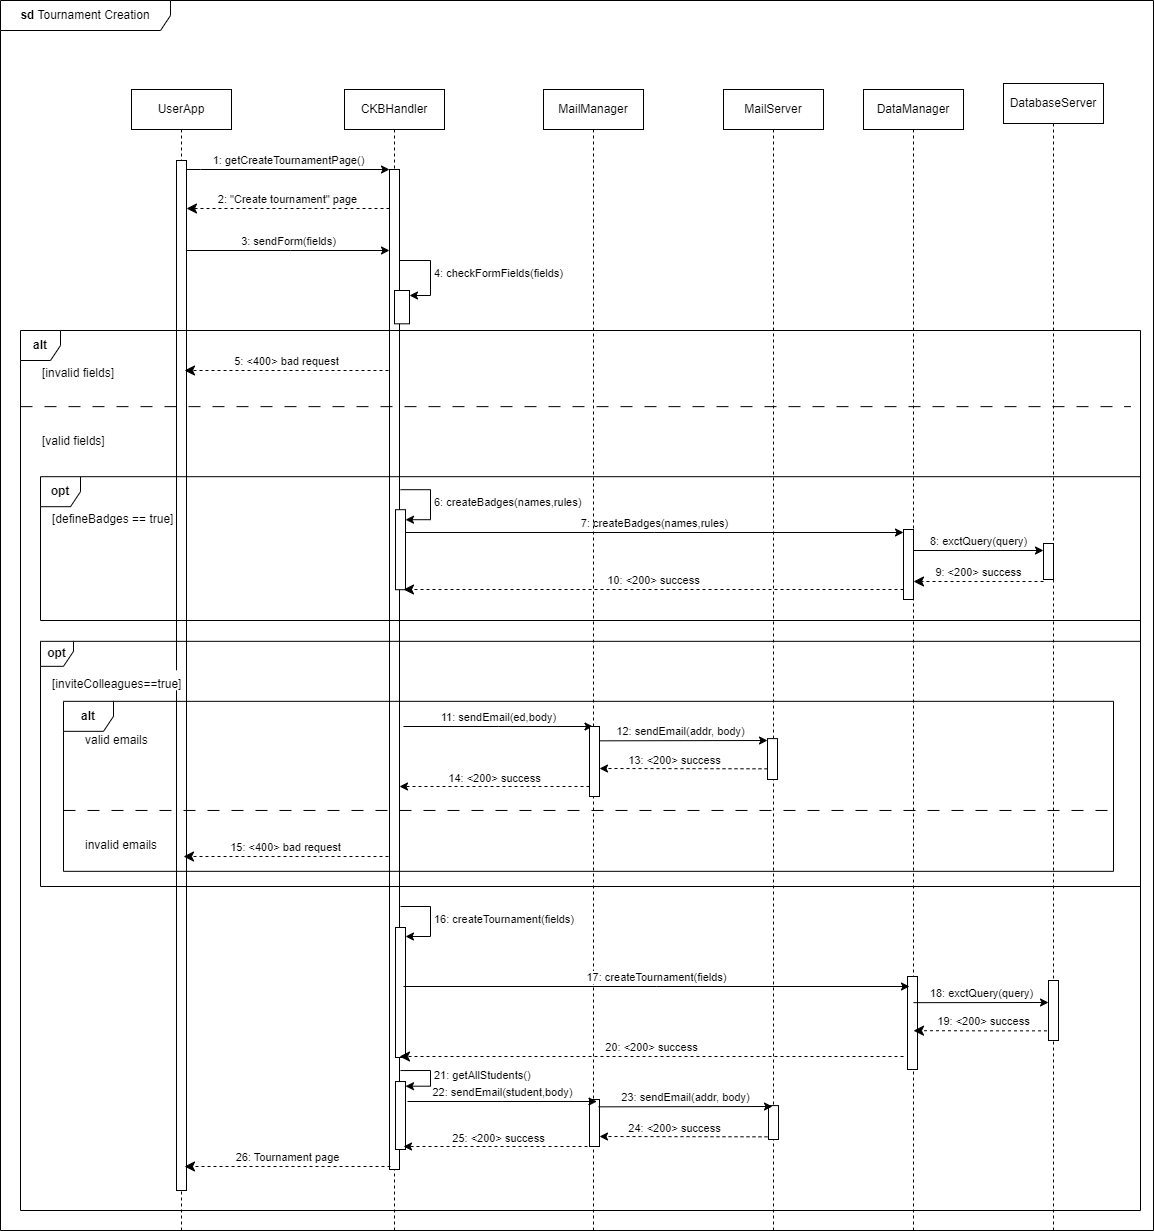
\includegraphics[width=1\textwidth]{images/seq_diagrams/tournament_creation_DD.png}
    \caption{Creation of the tournament}
\end{figure}
\clearpage

\subsection{Creation of the battle}
The figure below shows the sequence diagram of the creation of a battle. After the educator clicked ok the "Create Battle" button, they compile the form
 with the battle details and submits it. The system checks if the data is valid. The battle is created, so the system sends an email to all 
 the students subscribed to the tournament.\\  
 
\begin{figure}[H]
    \centering
    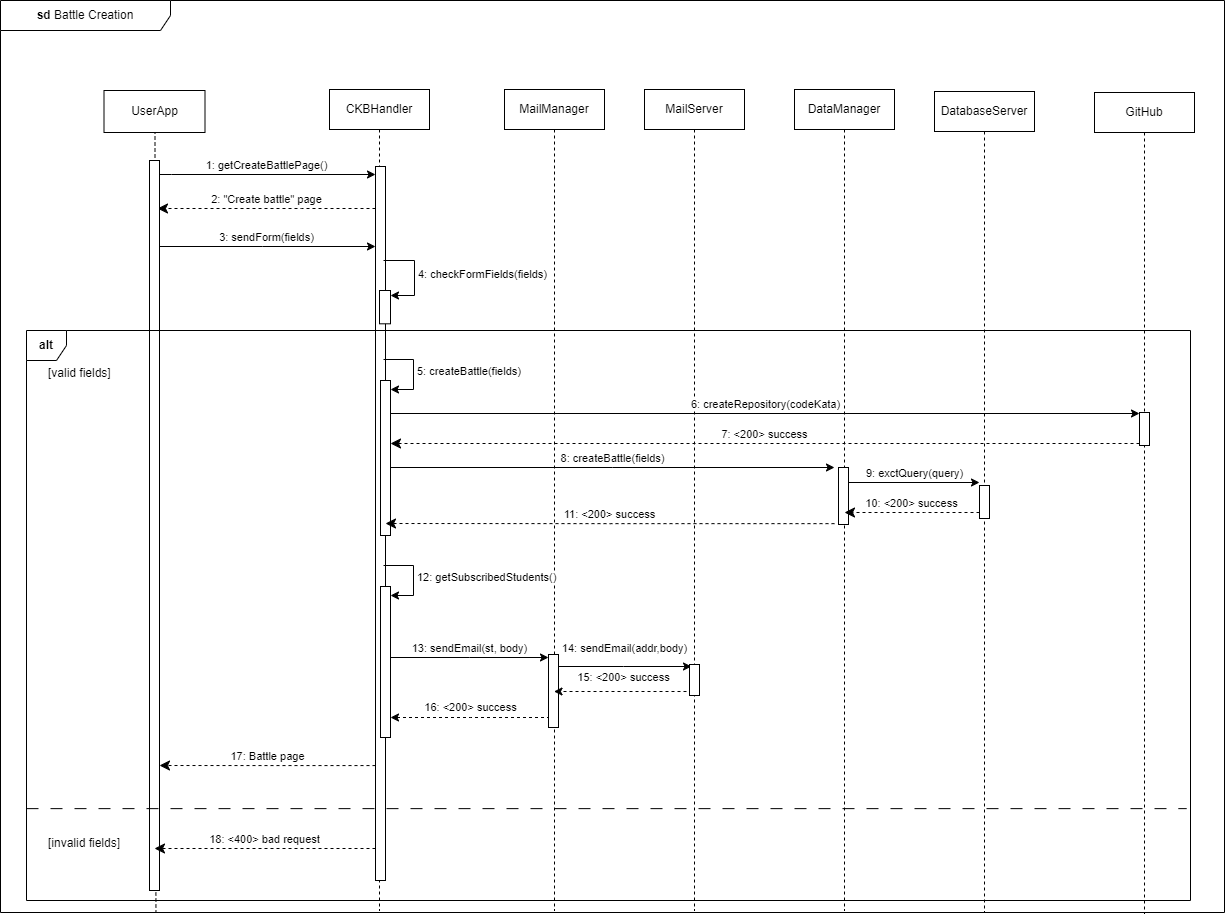
\includegraphics[width=1\textwidth]{images/seq_diagrams/battle_creation_DD.png}
    \caption{Creation of the battle}
\end{figure}
\clearpage

\subsection{Tournament visualization}
The figure below shows the sequence diagram of the visualization of a tournament. First the user requests the list of ongoing tournaments, 
then the user selects the tournament he wants to visualize.\\
\begin{figure}[H]
    \centering
    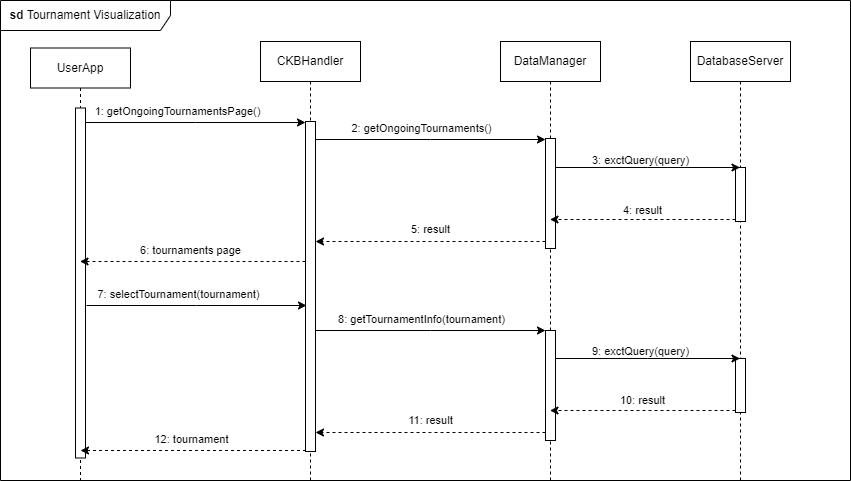
\includegraphics[width=1\textwidth]{images/seq_diagrams/tournament_visualization_dd.png}
    \caption{Tournament visualization}
\end{figure}
\clearpage

\subsection{Joining a tournament}
The figure below shows a student signing up for a tournament and receiving an email notification about it.\\
\begin{figure}[H]
    \centering
    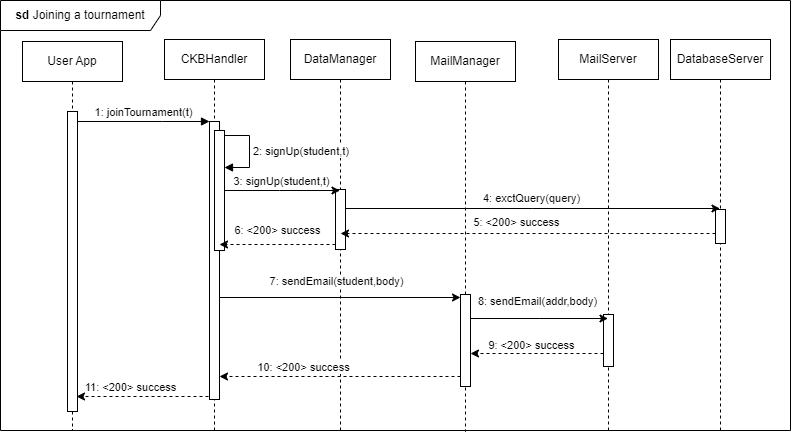
\includegraphics[width=1\textwidth]{images/seq_diagrams/joining_tournament_DD.png}
    \caption{Joining a tournament}
\end{figure}
\clearpage

\subsection{Joining a battle as a singleton}
The figure below shows a student joining a battle as a singleton and receiving an email notification about it. We assume that 
the battle configuration allows students to participate on their own.\\
\begin{figure}[H]
    \centering
    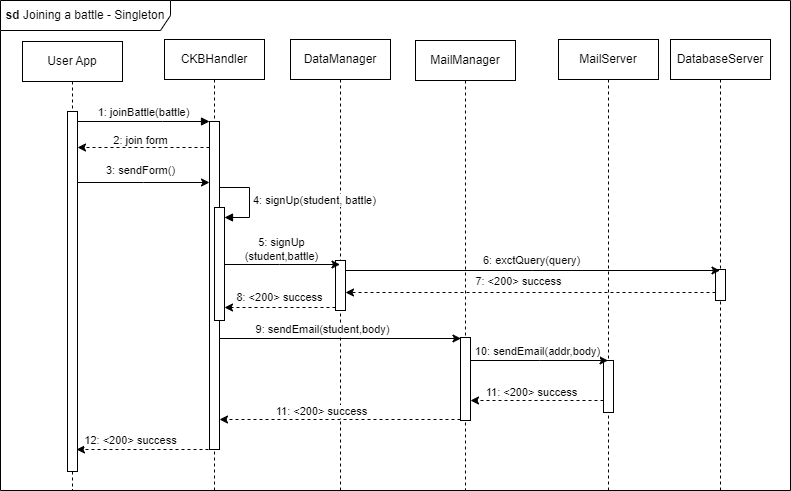
\includegraphics[width=1\textwidth]{images/seq_diagrams/joining_battle_singleton_DD.png}
    \caption{Joining a battle as a singleton}
\end{figure}
\clearpage

\subsection{Joining a battle by creating a group}
The figure below shows a student creating a group for a battle and receiving an email notification about it.\\
\begin{figure}[H]
    \centering
    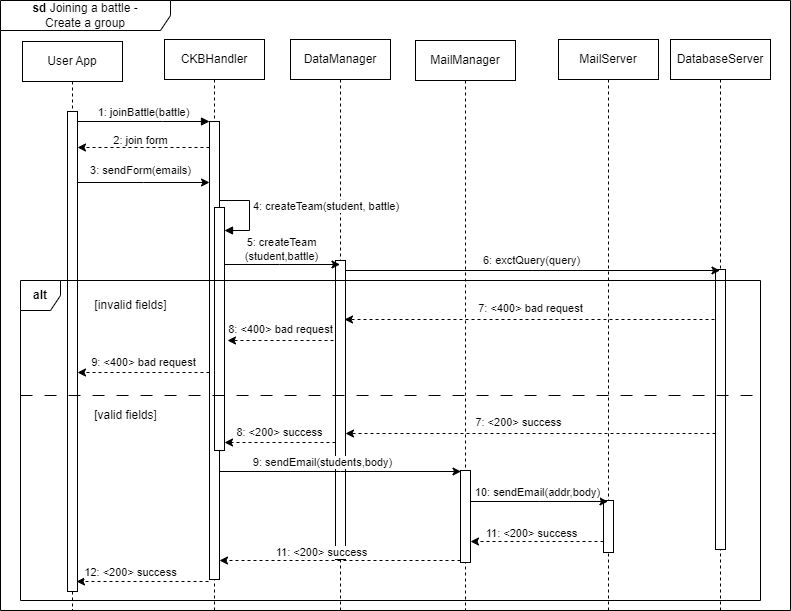
\includegraphics[width=1\textwidth]{images/seq_diagrams/joining_battle_create_group_DD.png}
    \caption{Joining a battle by creating a group}
\end{figure}
\clearpage

\subsection{Joining a battle by joining a group}
The figure below shows a student joining a group for a battle and receiving an email notification about it. If the 
minimum number of participants is reached, the team is signed up for the battle.\\
\begin{figure}[H]
    \centering
    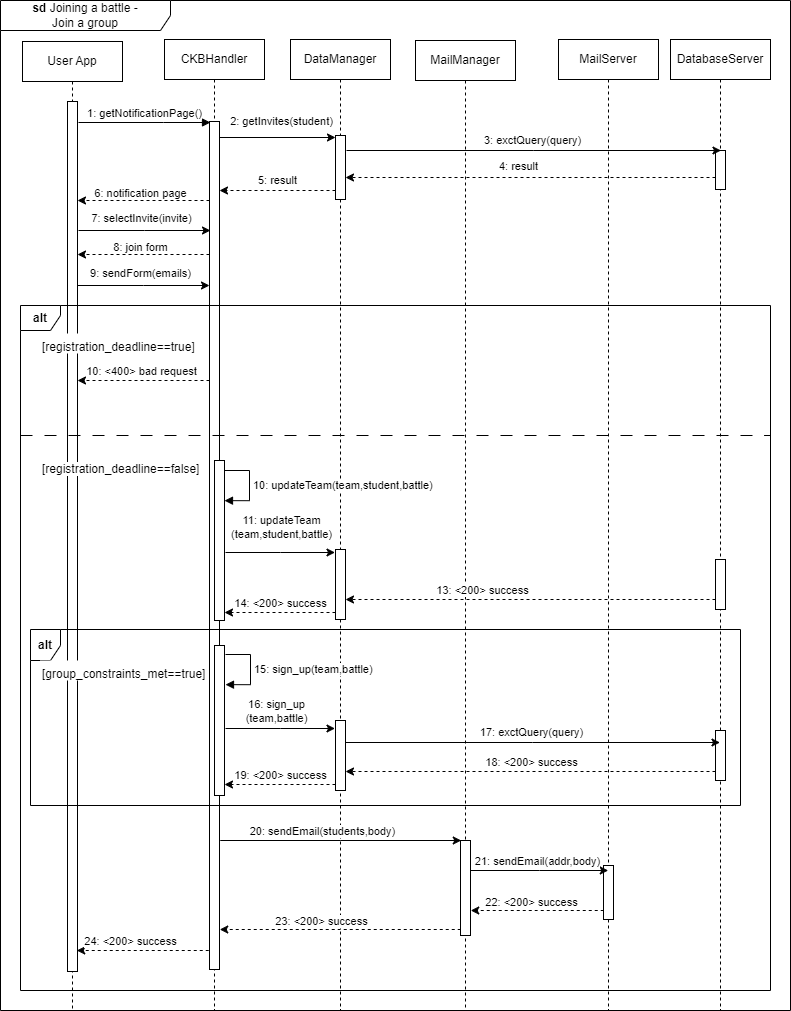
\includegraphics[width=1\textwidth]{images/seq_diagrams/joining_battle_join_group_DD.png}
    \caption{Joining a battle by joining a group}
\end{figure}
\clearpage

\subsection{Execution of the battle}
The figure below shows the sequence diagram of the execution of a battle. After GitHub notifies the system that a student pushed code, the system
evaluates automatically the code based on the requirements chosen by the educator at the creation of the battle and
updates the battle score of the student.\\
\begin{figure}[H]
    \centering
    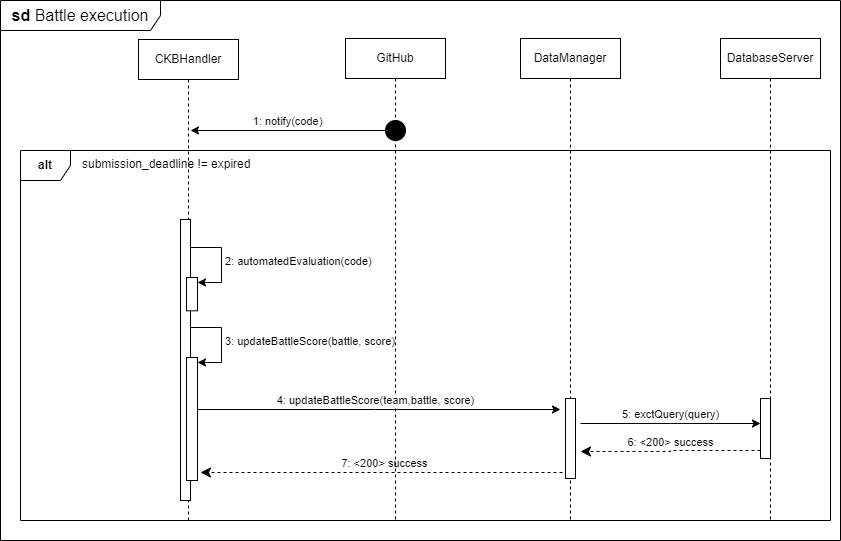
\includegraphics[width=1\textwidth]{images/seq_diagrams/battle_execution_DD.png}
    \caption{Execution of the battle}
\end{figure}
\clearpage

\subsection{Conclusion of the battle}
The figure below shows the sequence diagram of the conclusion of a battle. If required, the educator performs the manual evaluation and
the system updates the battle scores. Then, the system updates the tournament score of the students who participated in the battle and 
the tournament rank. The system sends an email to all the students subscribed to the tournament to notify them that the updated tournament 
rank is available.\\
\begin{figure}[H]
    \centering
    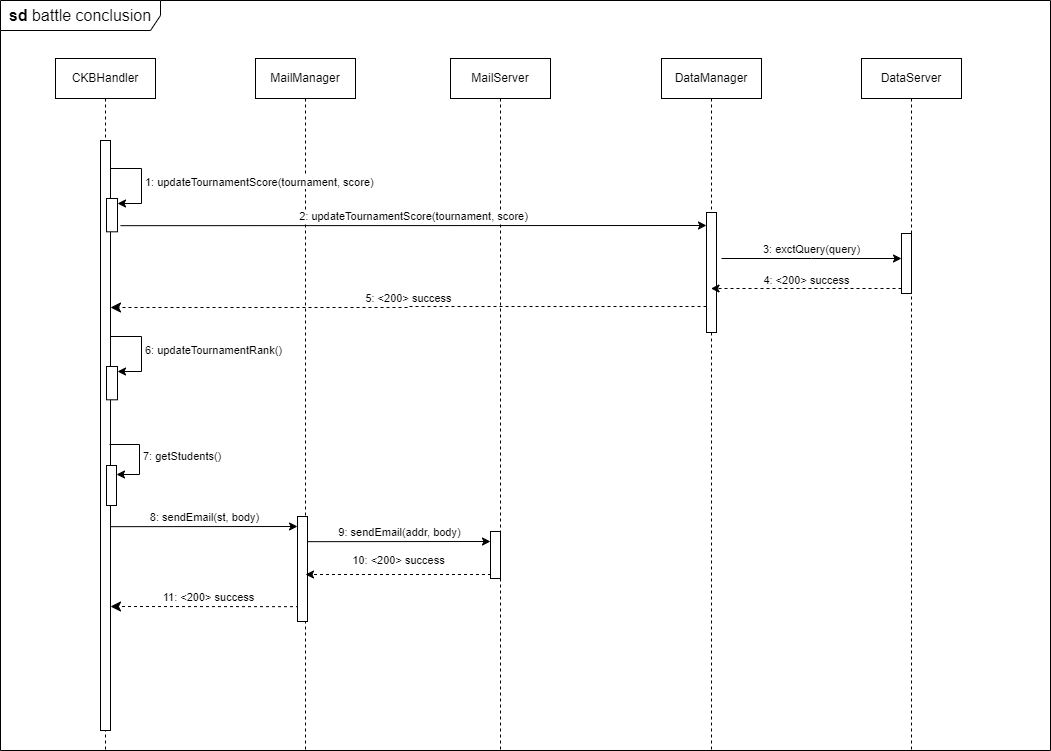
\includegraphics[width=1\textwidth]{images/seq_diagrams/battle_conclusion_DD.png}
    \caption{Conclusion of the battle}
\end{figure}
\clearpage

\subsection{Conclusion of a tournament}
The figure below shows the sequence diagram of the conclusion of a tournament. The educator chooses to conclude the tournament, so the system 
awards badges to students and sends an email notification to all subscribed students.\\
\begin{figure}[H]
    \centering
    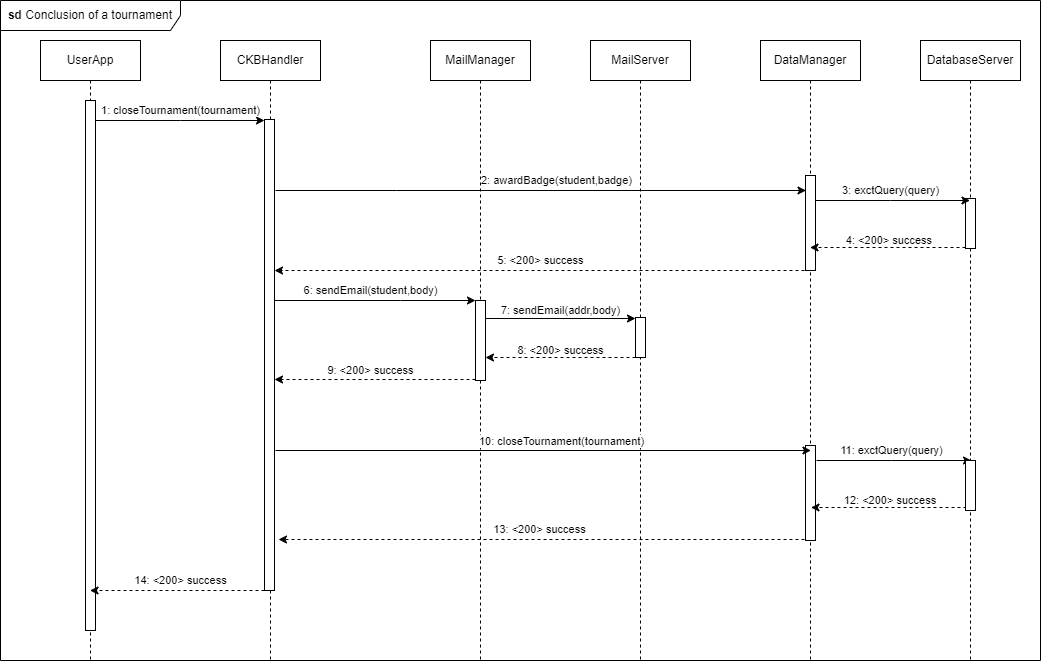
\includegraphics[width=1\textwidth]{images/seq_diagrams/tournament_conclusion_DD.png}
    \caption{Conclusion of a tournament}
\end{figure}
\clearpage

\subsection{Profile visualization}
The figure below shows the sequence diagram of the visualization of the profile of a student. 
The system retrieves the data of the searched student from the database if the student is registered to the system, otherwise it sends an 
error message.\\
\begin{figure}[H]
    \centering
    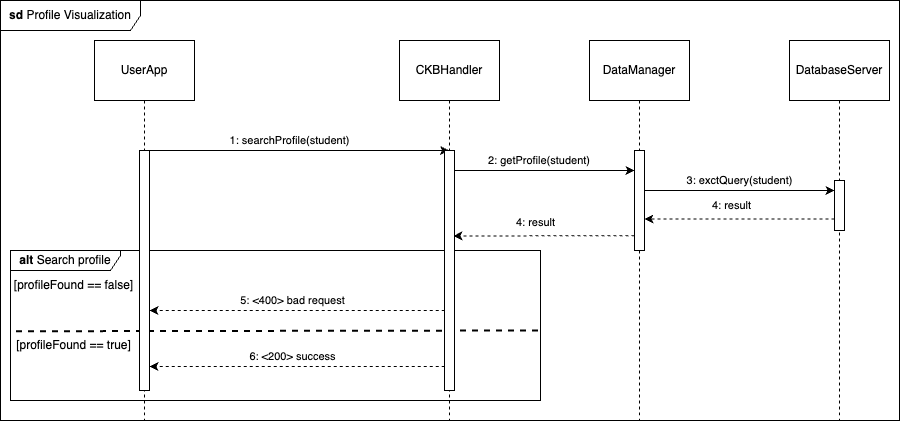
\includegraphics[width=1\textwidth]{images/seq_diagrams/ProfileVis_DD.png}
    \caption{Profile visualization}
\end{figure}
\clearpage

\section{Component interfaces}
In this section, the figure below depicts the interface diagram with the component interfaces and their specific methods and connections.
\begin{figure}[H]
    \centering
    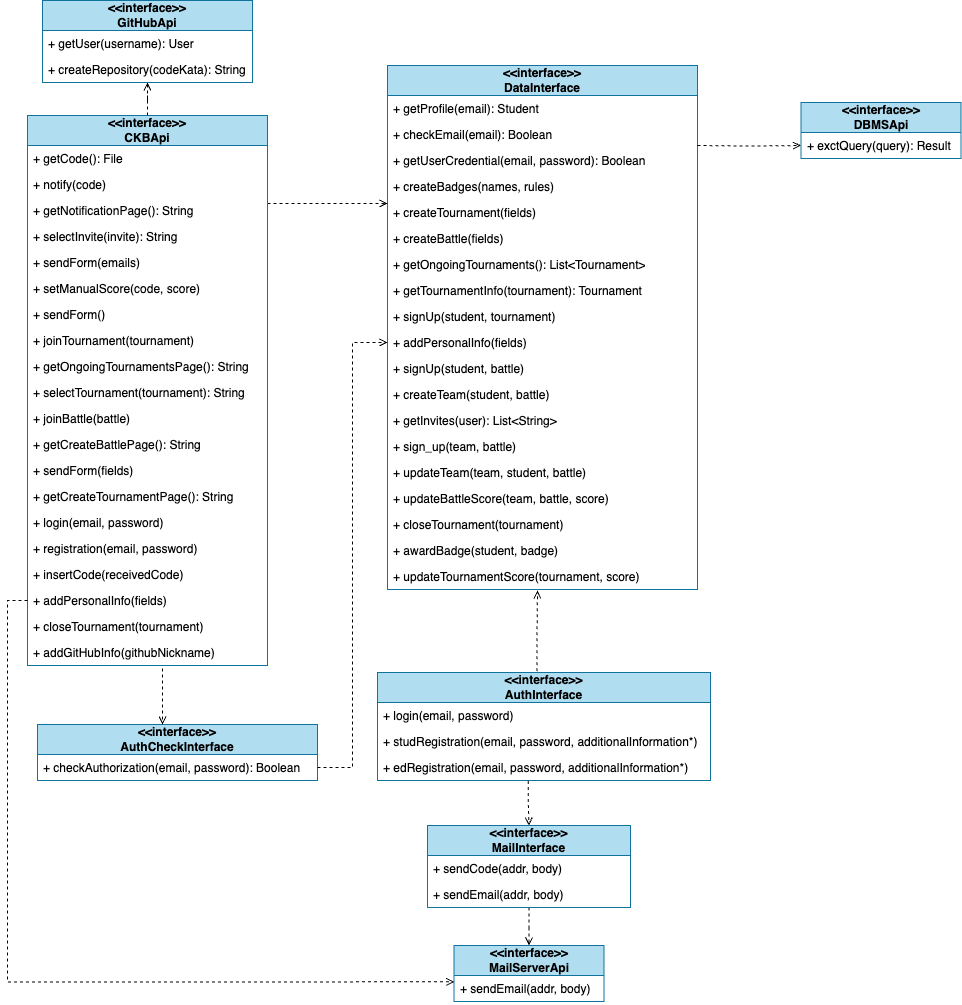
\includegraphics[width=1\textwidth]{images/Interface_diagram.png}
    \caption{Interface diagram}
\end{figure}
\clearpage

\section{Selected architectural styles and patterns}

\begin{itemize}
    \item \textbf{Three-tier architecture: }the system is based on a three-tier architecture, with every tier (presentation, application and data) 
    having a corresponding layer. The separation of the layers allows to scale the application efficiently by distributing the workload across 
    multiple servers. It also allows to improve the security of the system by protecting the data layer.
    Finally, it improves the maintainability of the system by allowing to modify a single layer without affecting the other ones.
    \item \textbf{REST architectural style: }the system is based on the REST architectural style. REST is a software architectural style that 
    defines a standard language for Web services. It is stateless and it makes easy to integrate with other systems thanks to the uniform 
    interface. It also allows for a clear separation between the client and the server. Client are not concerned with the internal state of the 
    server, promoting loose coupling and enhancing system maintainability.
\end{itemize}

\section{Other design decisions}

\subsection{ER diagram}
The figure below shows the Entity-Relationship diagram of the database used by the system.\\
\begin{figure}[H]
    \centering
    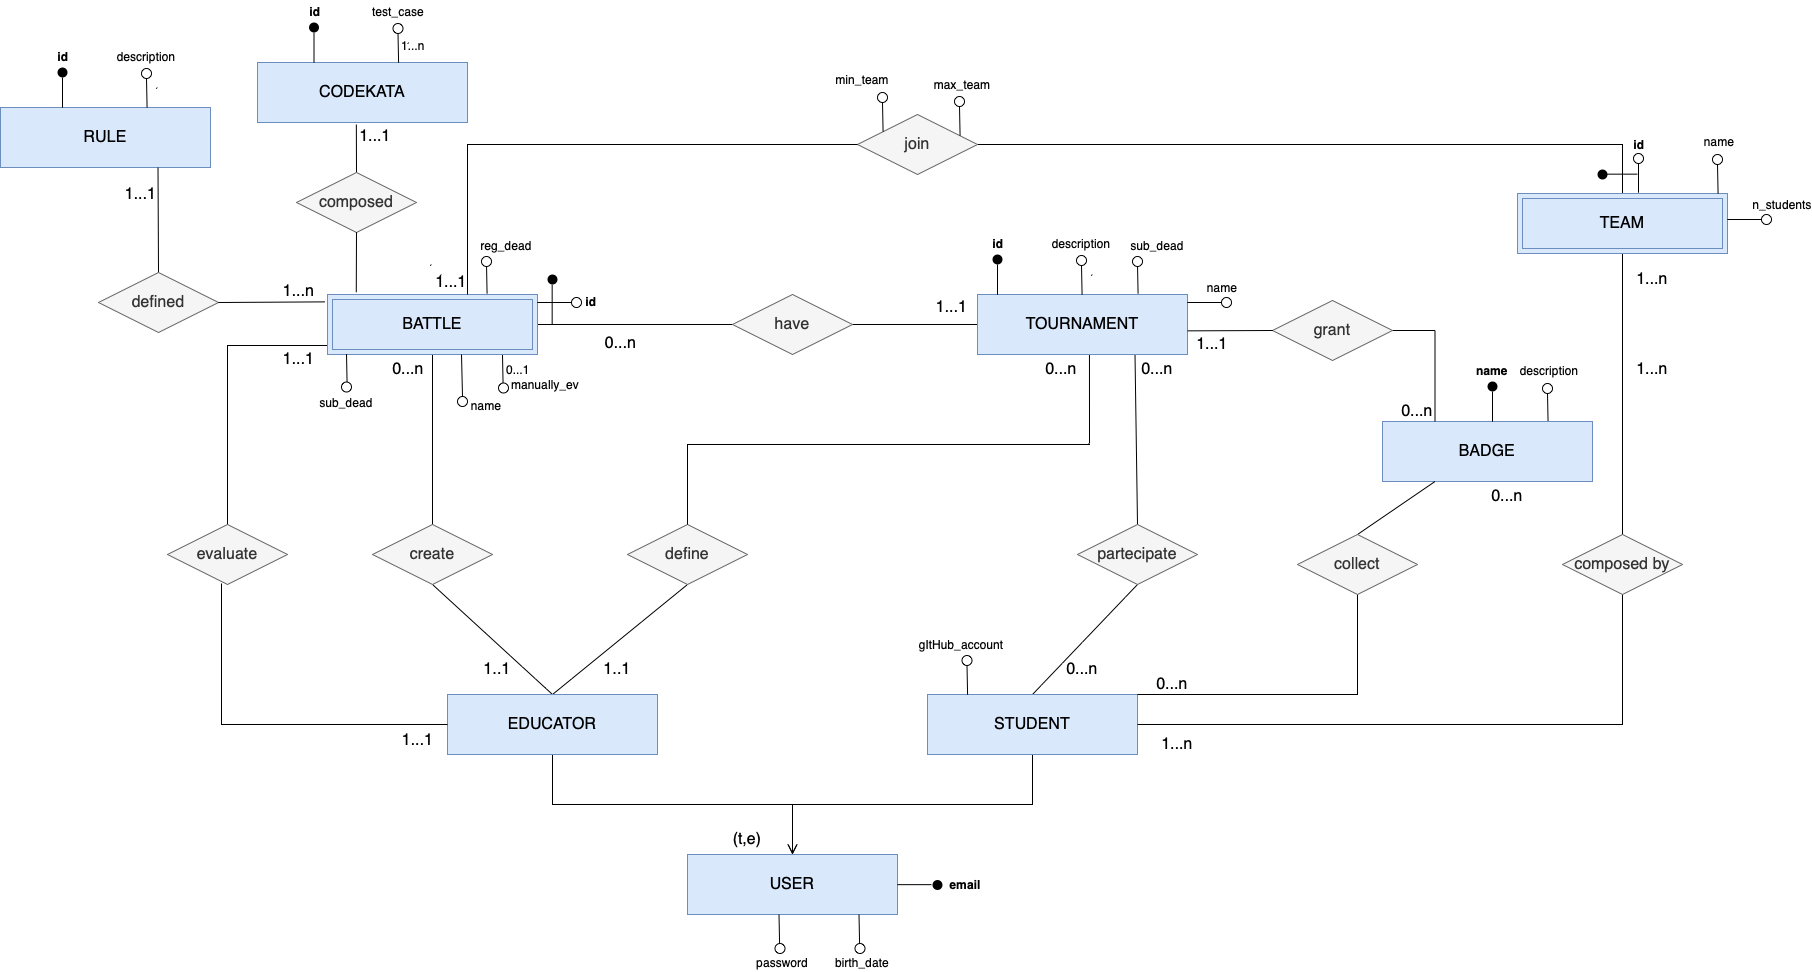
\includegraphics[width=1\textwidth]{images/ER_diagram.png}
    \caption{ER diagram}
\end{figure}